You will need to make some changes to your Cow Pi circuit before you can start this lab.

\subsection{Necessary Components}

Figure~\ref{fig:components} shows the components you will need for the range finder and alarm.

\begin{figure}
    \centering
    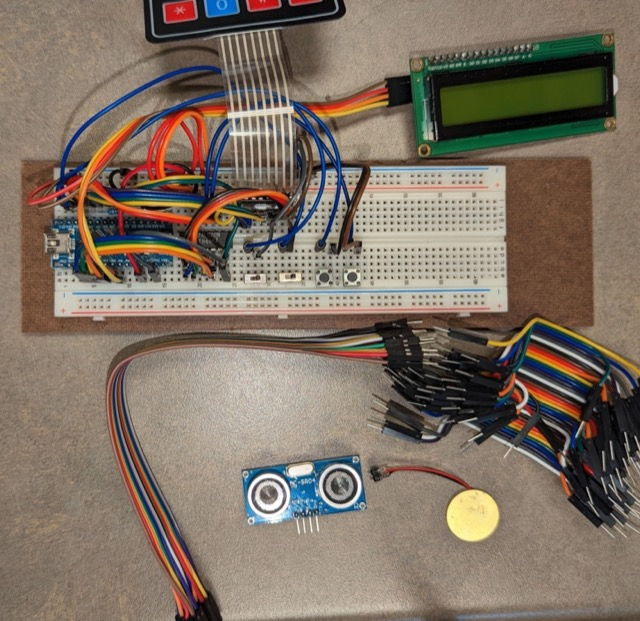
\includegraphics[width=10cm]{reconfiguration_images/components}
    \caption{Components needed for the Range Finder \label{fig:components}}
\end{figure}

You will need:
\begin{itemize}
    \item Your Cow Pi hardware circuit
    \item A piezoelectric disc
        \begin{itemize}
            \item Piezoelectric devices can convert electric energy into mechanical energy, and vice-versa
            \item You will use a piezoelectric disc to create an audible alarm
        \end{itemize}
    \item An ultrasonic echo sensor
        \begin{itemize}
            \item The two prominent drums on this device are ultrasonic transducers, one of which converts electricity to 40kHz sound (well above the range of human hearing), and the other of which converts 40kHz sound into electricity
            \item You will measure the time between the ultrasound being transmitted and its reflecting being received to determine the distance to whatever is reflecting the ultrasound
        \end{itemize}
    \item Two 20cm male-to-male wires and (optionally) two additional male-to-male wires
\end{itemize}

You and your partner only need to modify one of your Cow Pis (but you may modify both).

\subsection{Connecting the Piezoelectric Disc}

The \developmentboard's pin D9 is currently used for the right pushbutton.
In the group project, we will use it to control the piezodisc.

\begin{description}
    \checkoffitem{Remove the \textbf{right pushbutton} (Figure~\ref{fig:removeButton}).}
    \checkoffitem{Insert the piezodisc's header into the breadboard (Figure~\ref{fig:insertPiezo}).}
        \begin{itemize}
            \item The piezodisc's black wire is inserted into the breadboard's contact point b43.
            \item The piezodisc's red wire is inserted into the breadboard's contact point b44.
        \end{itemize}
    \checkoffitem{As shown in Figure~\ref{fig:adjustPiezoWire}, move the wire that is currently inserted into contact point e41 to contact point e44.}
\end{description}

\begin{figure}
    \centering
    \subfloat[Removing the right pushbutton.]{
        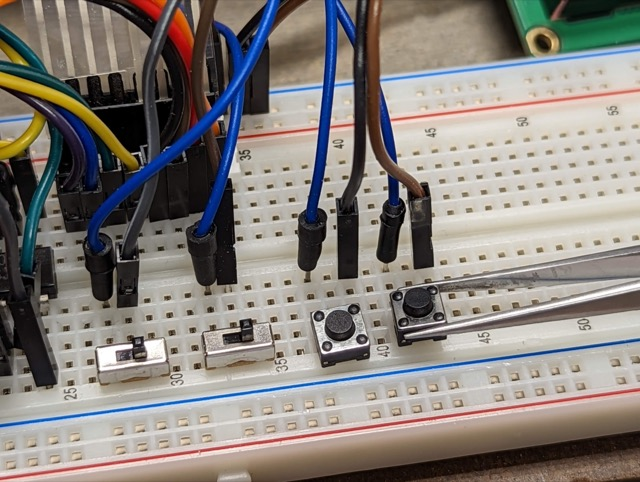
\includegraphics[height=4cm]{reconfiguration_images/remove_button}
        \label{fig:removeButton}
    }
    \hfil
    \subfloat[Inserting the piezodisc.]{
        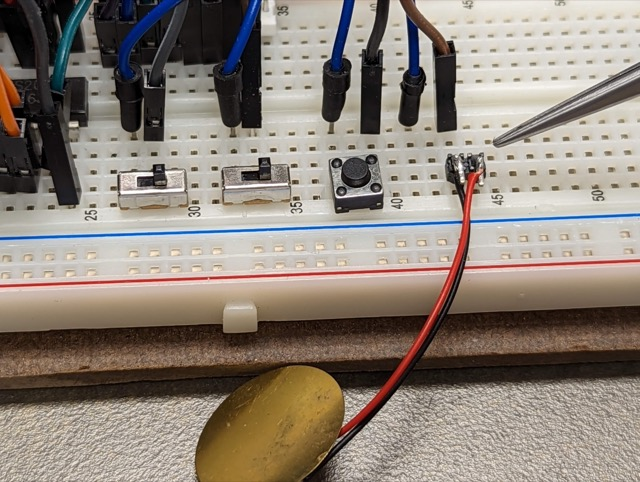
\includegraphics[height=4cm]{reconfiguration_images/insert_piezo}
        \label{fig:insertPiezo}
    }
    \hfil
    \subfloat[Adjusting the wiring for the piezodisc.]{
        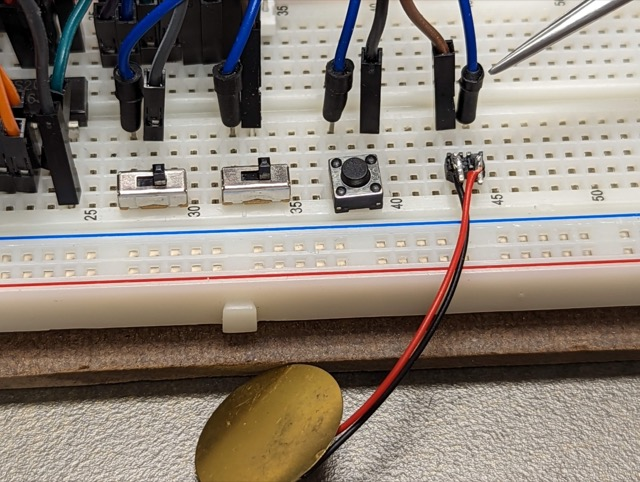
\includegraphics[height=4cm]{reconfiguration_images/adjust_piezo_wire}
        \label{fig:adjustPiezoWire}
    }
    \caption{Connecting the Piezoelectric Disc.
        The tweezers in these photos are to point out the changes and are not needed for \textit{these} modifications.}
\end{figure}

The piezodisc is now connected to the \developmentboard's pin D9, which is the pin that the right pushbutton used to be connected to.
The starter code will re-configure this pin to be an output pin.

\subsection{Connecting the ultrasonic echo sensor}

\begin{figure}
    \centering
    \subfloat[Locating the wires to remove.]{
        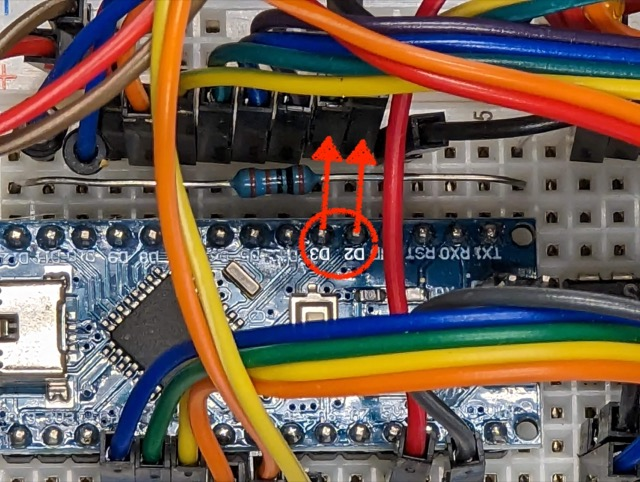
\includegraphics[height=4cm]{reconfiguration_images/pins_D2_D3}
        \label{fig:locateD2D3}
    }
    \\
    \subfloat[Removing the wire from contact point j10.]{
        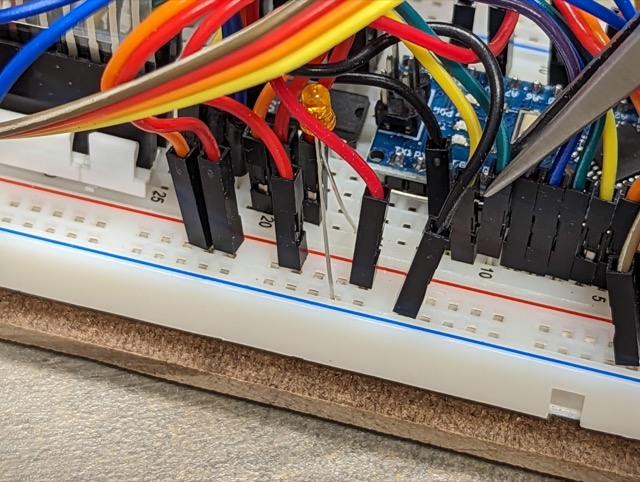
\includegraphics[height=4cm]{reconfiguration_images/remove_D3}
        \label{fig:removeD3}
    }
    \hfil
    \subfloat[Removing the wire from contact point j11.]{
        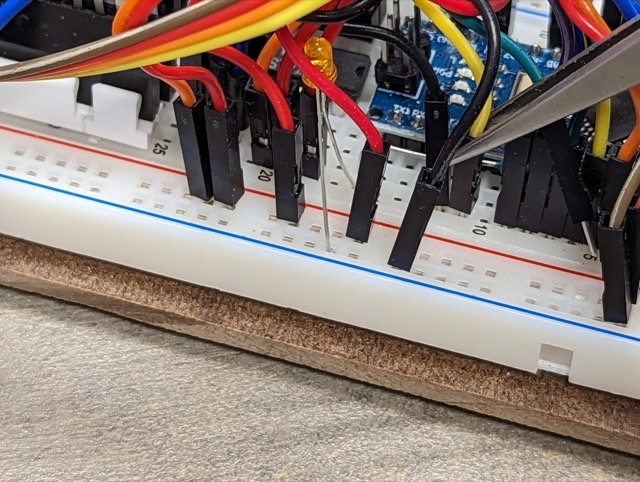
\includegraphics[height=4cm]{reconfiguration_images/remove_D2}
        \label{fig:removeD2}
    }
    \hfil
    \subfloat[An option is to leave the two wires hanging loosely.]{
        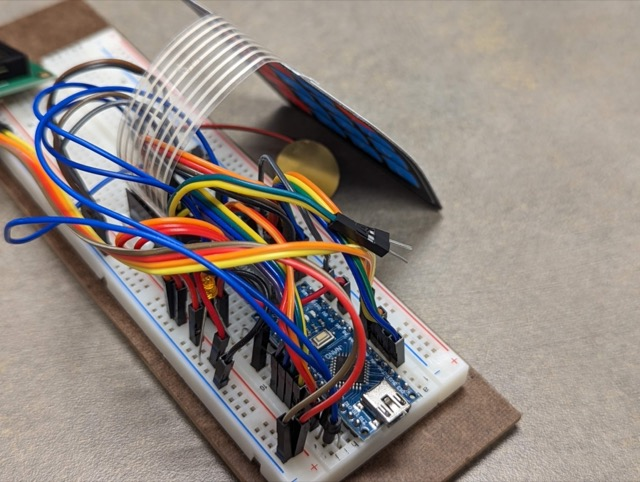
\includegraphics[height=4cm]{reconfiguration_images/NAND_wires_floating}
        \label{fig:nandFloat}
    }
    \hfil
    \subfloat[An option is to remove the wires completely from the breadboard.]{
        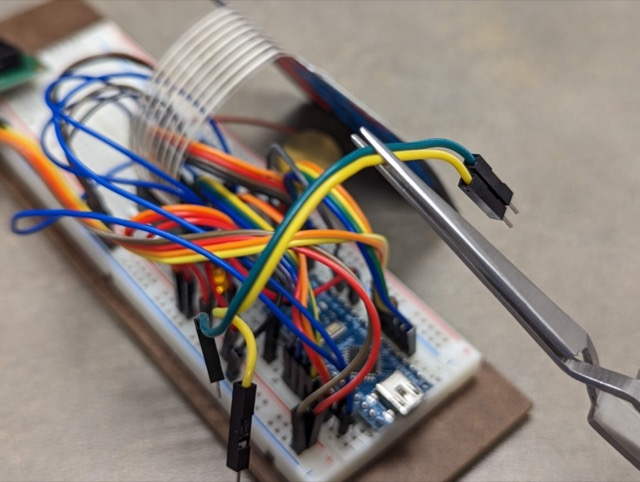
\includegraphics[height=4cm]{reconfiguration_images/NAND_wires_removed}
        \label{fig:nandRemoved}
    }
    \caption{Disconnecting the 74LS20 from the \developmentboard.}
\end{figure}

The \developmentboard's pins D2 \& D3 are currently used for the NAND values of the pushbuttons and of the keypad columns.
In the group project, we will use those pins for the ultrasonic echo sensor.

\subsubsection{Disconnecting the NAND} \label{subsubsec:disconnectNAND}

\textbf{\textit{Make sure that both you and your partner agree with which wires to pull before you do so!}}
If your partner is not available, then find someone to agree that you are about to pull the correct wires.

If you do not have the finger dexterity to remove the wires in the following steps with your fingertips, then the TAs will have a pair of needle-nose pliers during lab time that you can use.

\begin{description}
    \checkoffitem{Locate the wires that are connected to the \developmentboard's pins D2 \& D3 (Figure~\ref{fig:locateD2D3}).
        These are the wires in the breadboard's contact points j10 \& j11.}
    \checkoffitem{Gently remove the wire in the breadboard's contact point j10 (Figure~\ref{fig:removeD3}).}
    \checkoffitem{Gently remove the wire in the breadboard's contact point j11 (Figure~\ref{fig:removeD2}).}
    \checkoffitem{You may leave those two wires hanging loosely among the rat's nest of jumper wires, provided that they are positioned so they do not contact other components (Figure~\ref{fig:nandFloat}).
        Alternatively, you may \textit{very} gently tug at those two wires to completely remove them from the breadboard (Figure~\ref{fig:nandRemoved}).
        If you completely remove the wires, you can re-use them in Section~\ref{subsubsec:connectingSensor} to connect the ultrasonic echo sensor to the power and ground rails.}
\end{description}

\begin{figure}
    \centering
    \subfloat[Inserting a wire into contact point j11.]{
        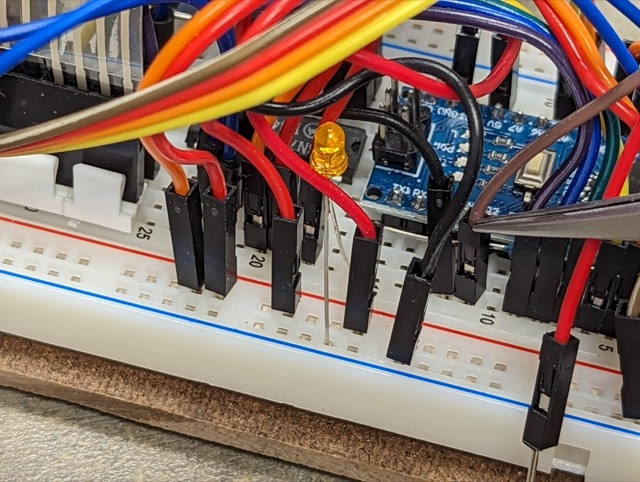
\includegraphics[height=4cm]{reconfiguration_images/insert_D2}
        \label{fig:insertD2}
    }
    \hfil
    \subfloat[Inserting a wire into contact point j10.]{
        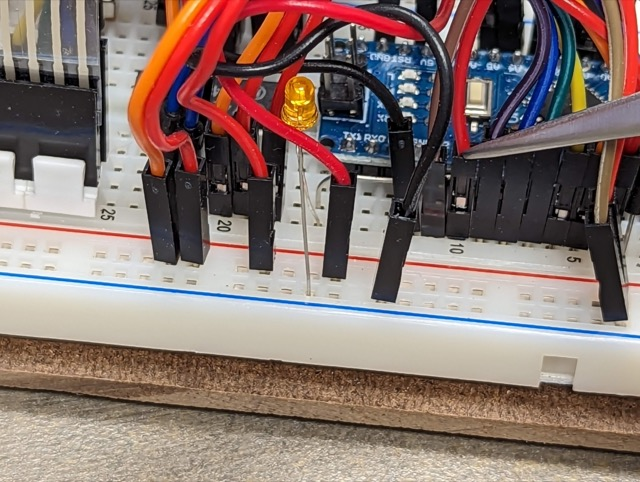
\includegraphics[height=4cm]{reconfiguration_images/insert_D3}
        \label{fig:insertD3}
    }
    \hfil
    \subfloat[The two 20cm wires, ready to be used.]{
        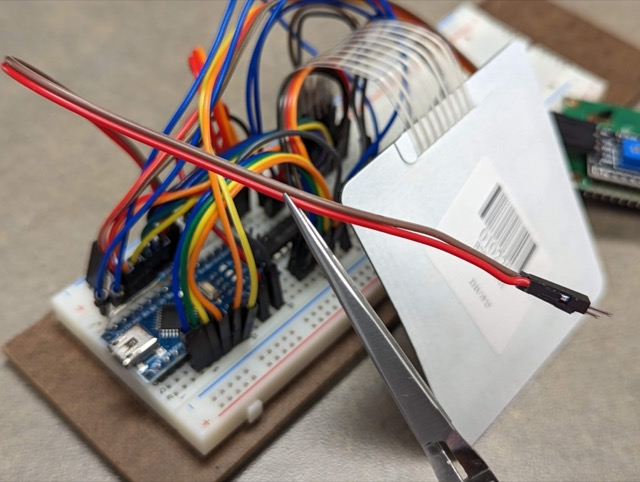
\includegraphics[height=4cm]{reconfiguration_images/20cm_D2_D3}
%        \label{fig:20cmD2D3}
    }
    \caption{Connecting the 20cm wires to the \developmentboard.}
\end{figure}

\subsubsection{Connecting the ultrasonic echo sensor} \label{subsubsec:connectingSensor}

You will first replace the NAND wires with 20cm male-to-male wires.

\begin{description}
    \checkoffitem{Insert a 20cm wire into contact point j11 (Figure~\ref{fig:insertD2}).
        Make a note of the wire's color for future reference.
        This is your \textbf{D2 wire}.}
    \checkoffitem{Insert a 20cm wire into contact point j10 (Figure~\ref{fig:insertD3}).
        Make a note of the wire's color for future reference.
        This is your \textbf{D3 wire}.}
\end{description}

Take a look at the ultrasonic echo sensor (Figure~\ref{fig:ultrasonic}).
Notice that it has four pins, labeled \texttt{Gnd}, \texttt{Echo}, \texttt{Trig}, and \texttt{Vcc}.

\begin{figure}
    \centering
    \subfloat[The back side of the ultrasonic sensor.]{
        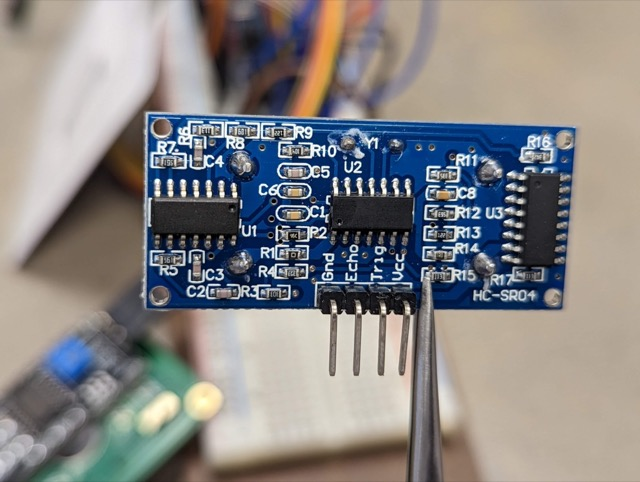
\includegraphics[height=4cm]{reconfiguration_images/ultrasonic_rear}
%        \label{fig:ultrasonicRear}
    }
    \hfil
    \subfloat[The front side of the ultrasonic sensor.]{
        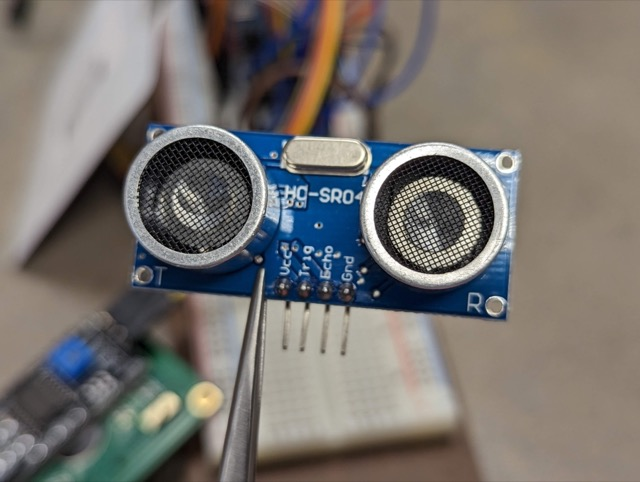
\includegraphics[height=4cm]{reconfiguration_images/ultrasonic_front}
%        \label{fig:ultrasonicFront}
    }
    \caption{The ultrasonic echo sensor. \label{fig:ultrasonic}}
\end{figure}

\begin{description}
    \checkoffitem{Insert the ultrasonic echo sensor in the breadboard's contact points d55--d58 (Figure~\ref{fig:ultrasonicInserted} shows the sensor in contact points e55--e58; however, testing shows slightly better results if the sensor's circuit board isn't allowed to dip into the breadboard's central channel).
        The \texttt{Gnd} pin should be in contact point d55, and the \texttt{Vcc} pin should be in contact point d58.
        The ultrasonic transducers should point toward the upper power/ground rails.}
    \checkoffitem{Insert the D2 wire into the breadboard's contact point b57, and the D3 wire into the breadboard's contact point b56 (Figure~\ref{fig:ultrasonicD2D3}).}
    \checkoffitem{Insert one end of a male-to-male wire in contact point b55 and the other end in the upper \ground.
        Insert one end of another male-to-male wire in contact point b58 and the other end in the upper \power.
        See Figures~\ref{fig:ultrasonicPwrGnd}--\ref{fig:pwrGnd}.
        If you fully-removed the wires between the 74LS20 and the \developmentboard\ in Section~\ref{subsubsec:disconnectNAND} then you can use those wires for this step (as we did in the photographs);
        otherwise, you will to use spare wires from your hardware kit.
        For best performance, position these wires so that they are not directly in front of the ultrasonic transducers.}
\end{description}

\begin{figure}
    \centering
    \subfloat[The back side of the ultrasonic sensor.]{
        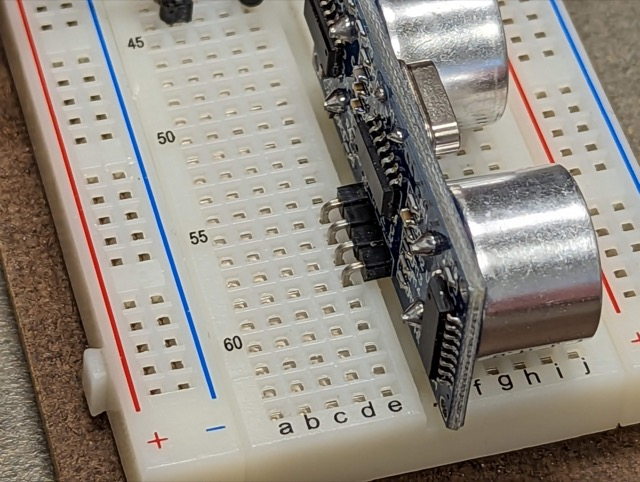
\includegraphics[height=4cm]{reconfiguration_images/ultrasonic_inserted}
        \label{fig:ultrasonicInserted}
    }
    \hfil
    \subfloat[The front side of the ultrasonic sensor.]{
        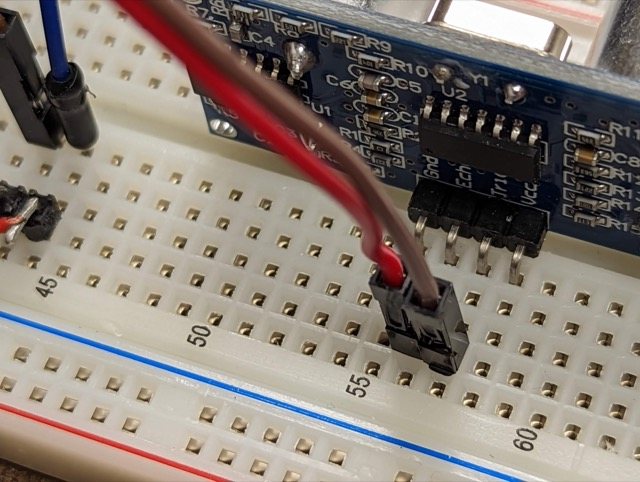
\includegraphics[height=4cm]{reconfiguration_images/ultrasonic_D2_D3}
        \label{fig:ultrasonicD2D3}
    }
    \hfil
    \subfloat[Inserting one end of the power and ground wires.]{
        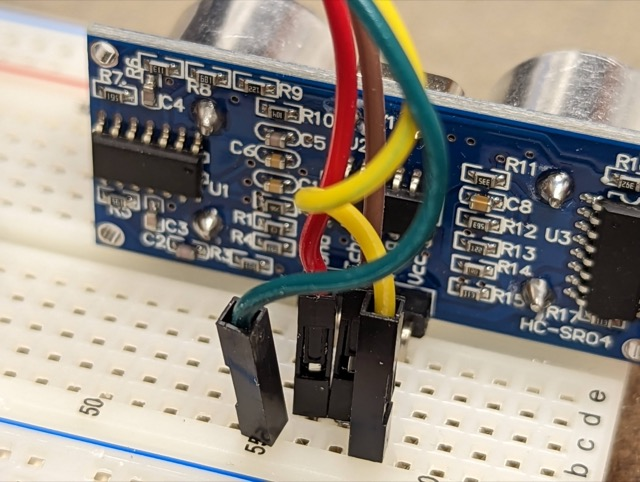
\includegraphics[height=4cm]{reconfiguration_images/ultrasonic_pwr_gnd}
        \label{fig:ultrasonicPwrGnd}
    }
    \hfil
    \subfloat[Inserting the other end of the power and ground wires in the power and ground rails.]{
        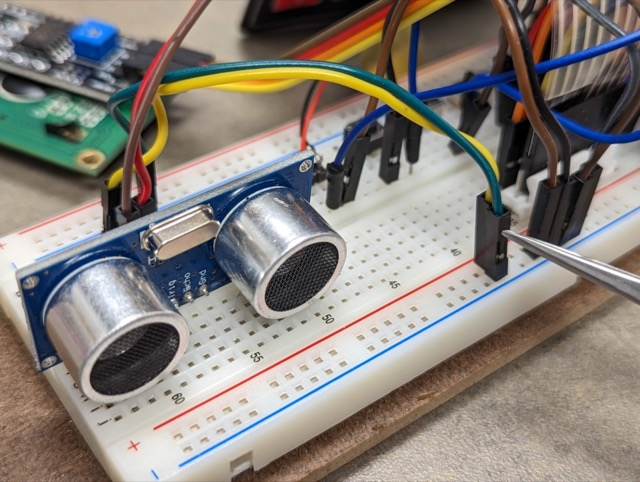
\includegraphics[height=4cm]{reconfiguration_images/pwr_gnd}
        \label{fig:pwrGnd}
    }
    \caption{Connecting the ultrasonic echo sensor.}
\end{figure}

The ultrasonic echo sensor is now connected to the \developmentboard's pins D2 \& D3.
The starter code will re-configure D2 to be an output pin.

\begin{figure}
    \centering
    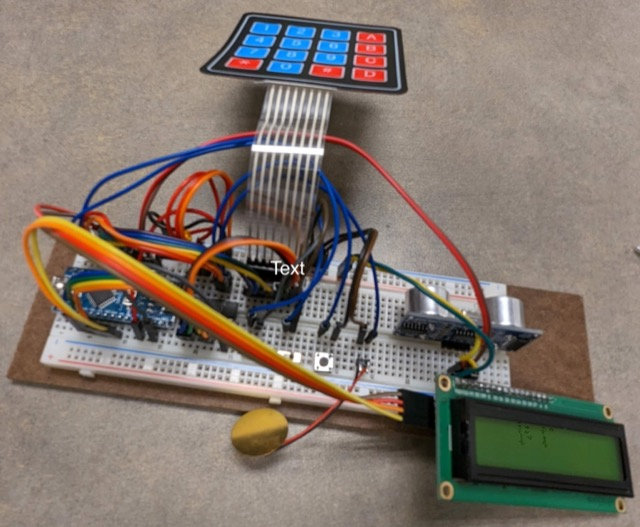
\includegraphics[width=10cm]{reconfiguration_images/complete}
    \caption{The Cow Pi circuit with modfications complete.}
\end{figure}

\vspace{1cm}

Your Cow Pi circuit is now ready for you to design and code the software for a range finder and alarm.
